%!TEX root = ../Thesis.tex
\section{Fazit (An-Nam Pham)}
\subsection{Fazit zur Consulting Lösung}
Das \acrfull{ITBA} trägt stark zur Business-Performance (Leistung des Unternehmens) bei.\\
In der Ausgangssituation des Unternehmens wurde die IT eher als notwendiges Mittel zum Ausführen von Arbeitsschritten eingesetzt. Die Gestaltung der IT-Landschaft glich einem Patchwork und überforderte die Mitarbeiter (vor allem die Mitarbeiter der IT-Abteilung).

Unsere Lösung hat das Ziel das ITBA zu optimieren und die IT dadurch nicht nur als notwendiges Werkzeug, sondern als starken Partner der Geschäftsführung einzusetzen.

Mit der Einführung eines SAP-Multichannel-Systems können dabei mehrere Fliegen mit einer Klappe geschlagen werden:
\begin{itemize}
\item Geschäfts- und IT-Prozesse nach ITIL sorgen für reibungsarmes Funktionieren des Unternehmens
\item Vereinfachter und optimierter IT-Support und IT-Administration
\item Entlastung der IT-Mitarbeiter
\item Verstärkung der Datensicherheit
\item Einsparungen von Kosten
\item Vertrieb, Marketing und Außendienst bekommen ein starkes Hilfsmittel, wodurch Mitarbeiter eingespart oder besser in ihrer Abteilung eingesetzt werden können (\glqq weniger Papierkram, mehr richtige Arbeit\grqq)
\item Verbessertes Arbeitsklima
\item etc.
\end{itemize}
\newpage

Die folgenden Abbildungen \ref{img:Fazit1} und \ref{img:Fazit2} zeigen den Vorher-Nachher-Vergleich:
\begin{figure}[H]
\centering
\begin{minipage}[t]{1\textwidth}
\fbox{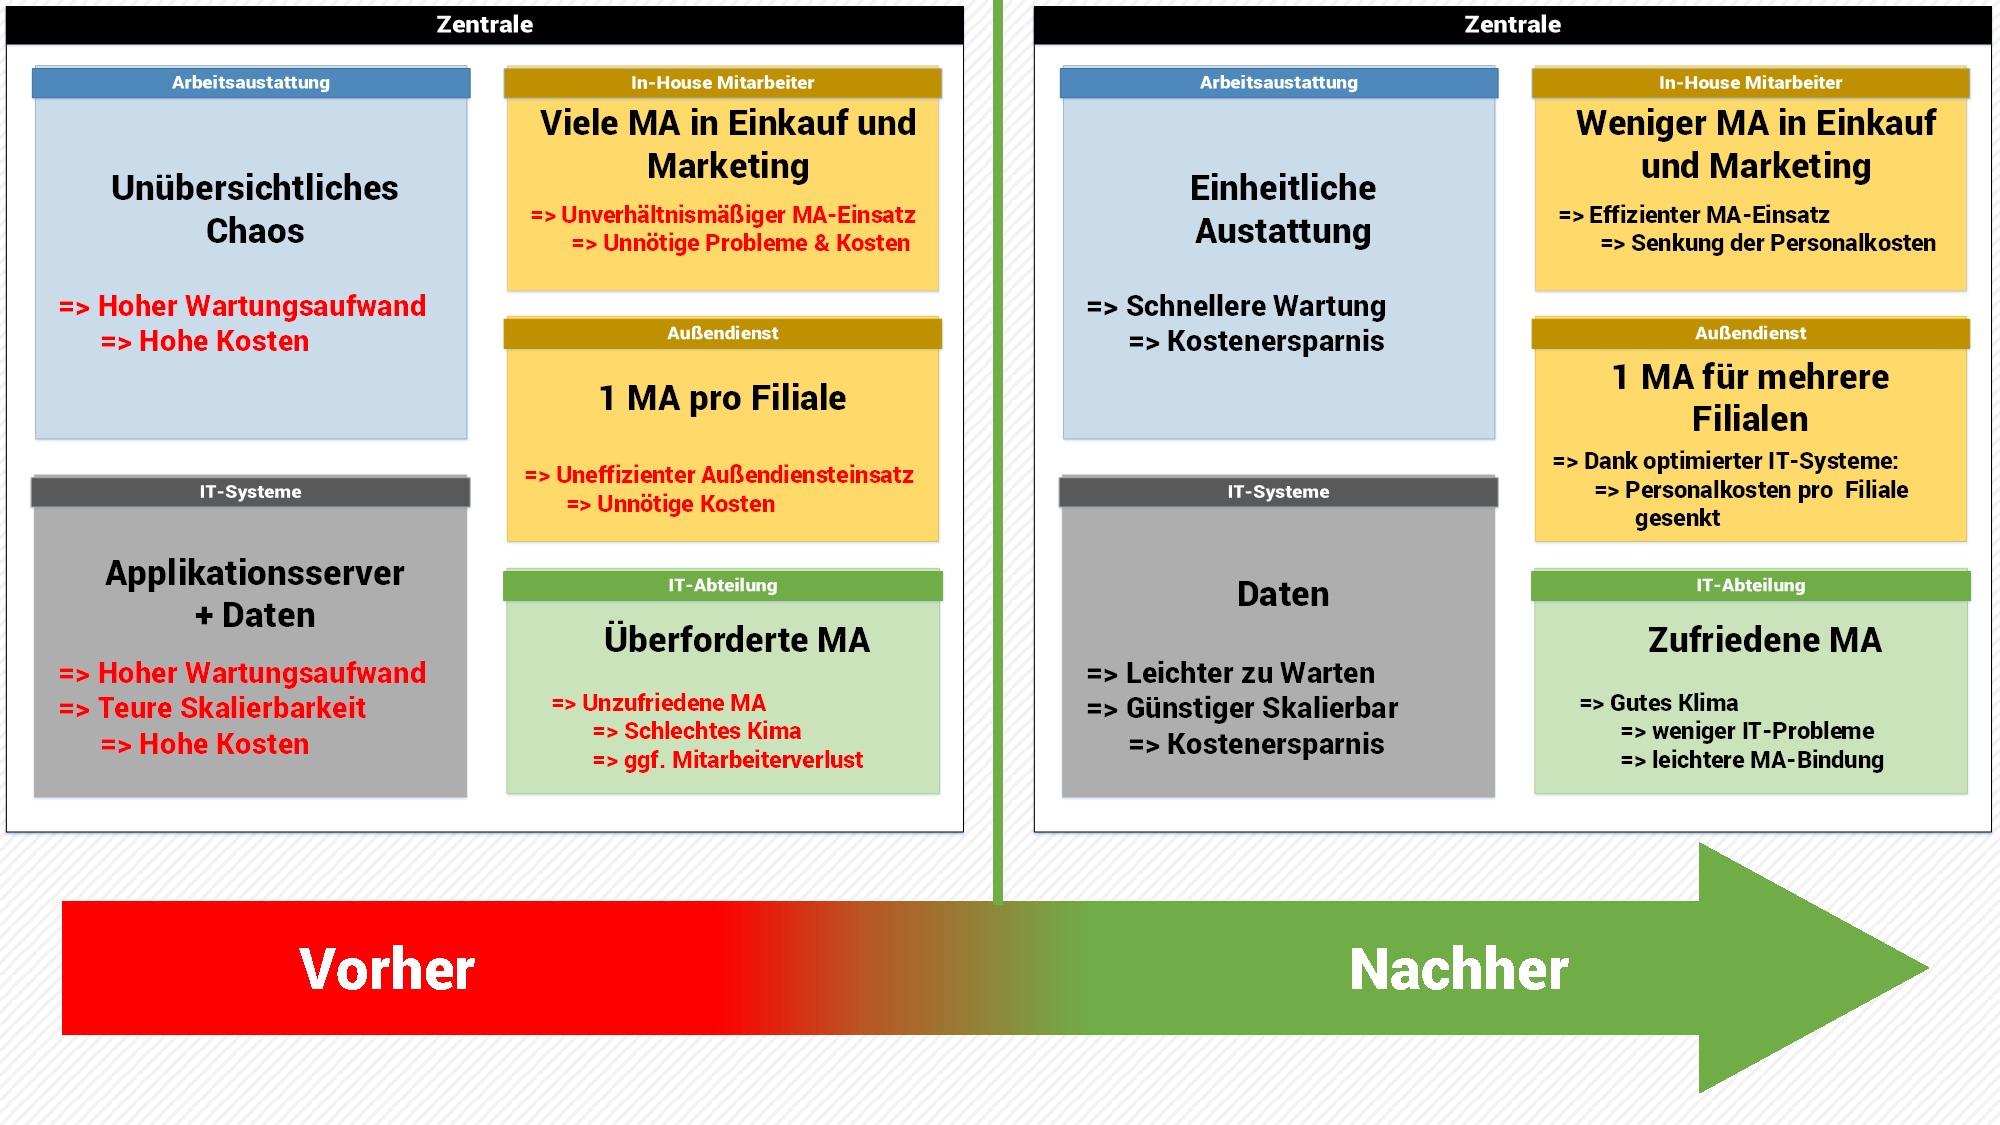
\includegraphics[width=1\textwidth,page=1]{img/Fazit.pdf}}
\caption{Vorher-Nachher-Vergleich 1} % Überschrift
\source{Eigene Darstellung} % Quelle
\label{img:Fazit1}
\end{minipage}
\end{figure}

\begin{figure}[H]
\centering
\begin{minipage}[t]{1\textwidth}
\fbox{\includegraphics[width=1\textwidth,page=2]{img/Fazit.pdf}}
\caption{Vorher-Nachher-Vergleich 2} % Überschrift
\source{Eigene Darstellung} % Quelle
\label{img:Fazit2}
\end{minipage}
\end{figure}
\newpage

Allerdings ist das IT-Business-Alignment nicht der einzige Faktor für den Unternehmenserfolg.
Auch die Total Costs of Ownership (Gesamtbetriebskosten) sind von großer Bedeutung. Es muss immer überlegt werden, was man selber tut und was man lieber auslagert. In diesem  Fall ist es der IT-Server. Wie im Kapitel \ref{sec: AWS_Rechnung} aus Seite \ref{sec: AWS_Rechnung} erläutert, ist es günstiger, den Applikationsserver in die Cloud (IaaS) auszulagern. Dies spart hohe Anschaffungs- und Haltungskosten.
\subsection{Problematik: Haltung der Geschäftsführung zur IT}
\begin{quote}
\textit{\enquote{IT soll funktionieren und dabei kostengünstig sein.}\\(Geschäftsführung)} 
\end{quote}
Auch wenn wir als IT-Consultants nicht die Aufgabe hatten, den Job des Geschäftsführers zu verbessern oder zu kritisieren, muss unserer Meinung nach trotzdem kurz darauf eingegangen werden.
Schließlich soll nicht nur das Problem, sondern auch die Ursache für das Problem bekämpft werden. Und die Geschäftsführung ist ein Teil der Ursache.

Es ist wichtig, dass die Geschäftsführung die IT nicht als \glqq notwendiges Übel\grqq~sieht, sondern als leistungsstarken Partner.

Anhand eines kurzen Beispiels soll dies deutlich gemacht werden:\\ 
An einem zufälligen Tag fällt die komplette IT aus (z.B. durch Servercrash oder einfachen Stromausfall).

Die Firma hat nun ein großes Problem. Jeder Mitarbeiter ist von der IT-Austattung und den Mitarbeitern der IT-Mitarbeiter abhängig.\\
Aus diesem Grund muss die IT von der Geschäftsführung gut gepflegt werden.

Dank Hochverfügbarkeits-Strategien von SAP und dem Cloud-Anbieter kann auf jeden Fall sichergestelt werden, dass die IT nur mit einer sehr geringen Wahrscheinlichkeit ausfallen kann.\\
Dafür muss die Cloud und SAP aber erstmal eingeführt werden.

Dies zeigt, dass dringendes Handlungsbedarf beim Unternehmen Stylez besteht. Und es sollte darüber nachgedacht werden, warum die Geschäftsführung erst gehandelt hat, nachdem sie von den IT-Mitarbeitern dazu gedrängt wurden.

Unserer Meinung nach muss die Geschäftsführung den Mehrwert der IT erkennen, um die IT langfristig gut pflegen zu können. Denn eine starke IT kann in der jetzigen Zeit, wo Geschwindigkeit entscheidend ist, enorme Wettbewerbsvorteile bringen.

Der Wettbewerb im Markt kann mit einem Schachspiel verglichen werden:\\
Man kann bei einem Schachspiel nur mit Bauern spielen. Es kann gut gehen, muss aber nicht. Außerdem ist dies sehr aufwändig und verzeiht keine strategischen Fehler.\\
Werden aber auch wertvollere (und stärkere) Figuren eingesetzt, lässt sich eine starke Strategie formen, um das Spiel zu gewinnen.

Die Geschäftsführung muss also entscheiden: Schwache Figuren einsetzen, oder den Vorteil stärkerer Figuren nutzen...

\subsection{Problematik: Multichannel vs. Franchisenehmer}
Bevor wir zur Problematik eingehen noch eine Anmerkung:\\
Auch hier mischen wir uns wieder in die Geschäftsführung ein. Wir wollen aber kurz auf die folgende Problematik eingehen, da das Multichannel-System dabei helfen kann, dieses Problem zu entschärfen.

Der Multichannel-Vertrieb bietet dem Kunden viele Vorteile: Er kann verschiedene Vertriebswege nutzen. Beispiele:
\begin{itemize}
\item Stöbern und Bestellen im Webshop $\rightarrow$ Bestellbestätigung per SMS und E-Mail $\rightarrow$ Rechnung per E-Mail $\rightarrow$ Abholung und Anprobe in der Filiale
\item Stöbern, Beratung und Kaufen in der Filiale $\rightarrow$ Rechnung per E-Mail $\rightarrow$ Stornierung per Webshop $\rightarrow$ Zurückgabe per Post
\end{itemize}
Es gibt unzählige Varianten der Vertriebswege, was dem Kunden eine hohe Flexibilität bietet. Dadurch steigt die Kundenzufriedenheit.

Allerdings steigt durch den Multichannel-Vertrieb nicht unbedingt die Zufriedenheit der Franchise-Nehmer.\\
Statistiken zeigen, dass die Beliebtheit des Online-Shoppings immer weiter steigt. Nicht nur aufgrund von günstigeren Preisen. Hauptsächlich auch aus Bequemlichkeit.

\textbf{Das große Problem:}\\
Der Franchisenehmer macht Umsatz, indem Kunden in seiner Filiale einkaufen.\\
Was aber, wenn der Kunde im Onlineshop kauft? Dann kann der Franchisenehmer keinen Umsatz generieren. Es kann auch vorkommen, dass ein Kunde ein Kleidungsstück im Webshop kauft, aber in der Filile umtauschen möchte (z.B. weil die Größe nicht passt). Oder wenn der Kunde online einkauft und auch online bezahlt, die Waren aber in der Filiale abholt? Dann macht der Franchisenehmer keinen Umsatz, obwohl Arbeitszeit und andere Aufwendungen dafür aufgewendet wurden.

Diese Problematik kann dafür sorgen, dass das Franchisemodell von Stylez unattraktiv wird und das Unternehmen ein Mangel an Franchisenehmern haben wird. Im schlimmsten Fall sogar Franchise-Nehmer verlieren wird. Und ohne Filialen wird der Einkauf bei Stylez für den Kunden unattraktiver und das neu eingeführte Multichannel-System wird auf Dauer auch überflüssig.

\textbf{Mögliche Lösung:}\\
Eine mögliche Lösung kann das Multichannel-System bieten. Es kann z.B. bei einer Bestellung im Webshop prüfen, welche Filiale am nächsten zum gewünschten Lieferort ist. Von dieser Filiale soll dann die bestellte Ware geliefert werden.

Oder wenn ein Online-Einkauf an eine Filiale geliefert werden soll, dann soll der Erlös an die Filiale und nicht an die Zentrale gehen.

Auch Provisionen vom Gesamtumsatz sind denkbar.

Diese Beispiele und noch viele andere Möglichkeiten lassen sich mit dem Multichannel-System umsetzen.

Wichtig ist aber, dass diese Problematik dem Unternehmen bewusst ist, und dass sie sich Gedanken machen, wie diese Probleme gelöst werden können.